\section{Resultate}

Es  gibt  ein  paar  interessante  Simulationen,  die  durchgef\"uhrt   werden
k\"onnen.

\subsection{Unm\"oglicher Sollwert}

Wie bereits in der Theorie erl\"autert, nimmt die  Drehzahl  des Motors linear
mit dem Lastmoment ab. Das heisst also, dass der Motor  die  maximale Drehzahl
von 1000 U/min nur erreichen kann, wenn keine Last vorhanden ist.

Es   wird   eine  Last  von  \SI{0.005}{\newton\meter\per(\radian\per\second)}
simuliert und der Sollwert wird auf 1000 U/min gesetzt.

\begin{figure}[H]
    \centering
    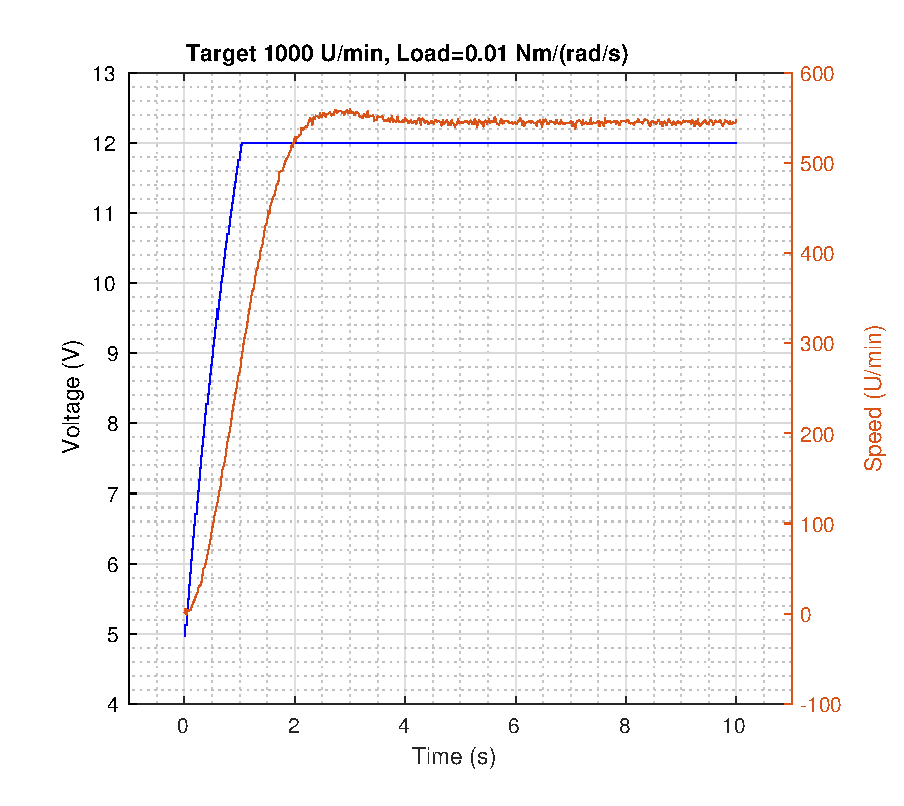
\includegraphics[width=\imagewidth]{images/target_1000_load_10}
    \caption{Verhalten bei einem Sollwert von 1000 U/min und einer Last von \SI{0.01}{\newton\meter\per(\radian\per\second)}. Es werden nur 545.3 U/min erreicht.}
    \label{fig:target_1000_load_10}
\end{figure}

Wir sehen in der Abbildung \ref{fig:target_1000_load_10} dass nur gerade 545.3
U/min  erreicht  werden,  und  die  Eingangsspannung  des  Motors  bleibt  bei
\SI{12}{\volt}  h\"angen  (der  PID-Regler  wurde  so  eingestellt,  dass  die
Ausgangsspannung limitiert wird).


\subsection{Windup}

Diese   Spannungslimitierung  (engl.  \textit{Clamping})  f\"uhrt   zu   einer
Nicht-Linearit\"at  im Regelkreis und es kann zu einem  ``Aufwickeln''  (engl.
\textit{Windup}) f\"uhren. Dabei wird der  Integralteil  des PID-Reglers immer
gr\"osser  und gr\"osser, was zur Folge  hat,  dass  bei  der  Entfernung  der
St\"orgr\"osse der Regler nicht sofort reagiert.

Dieses Verhalten ist gut in der Abbildung \ref{fig:windup} zu sehen.

\begin{figure}[H]
    \centering
    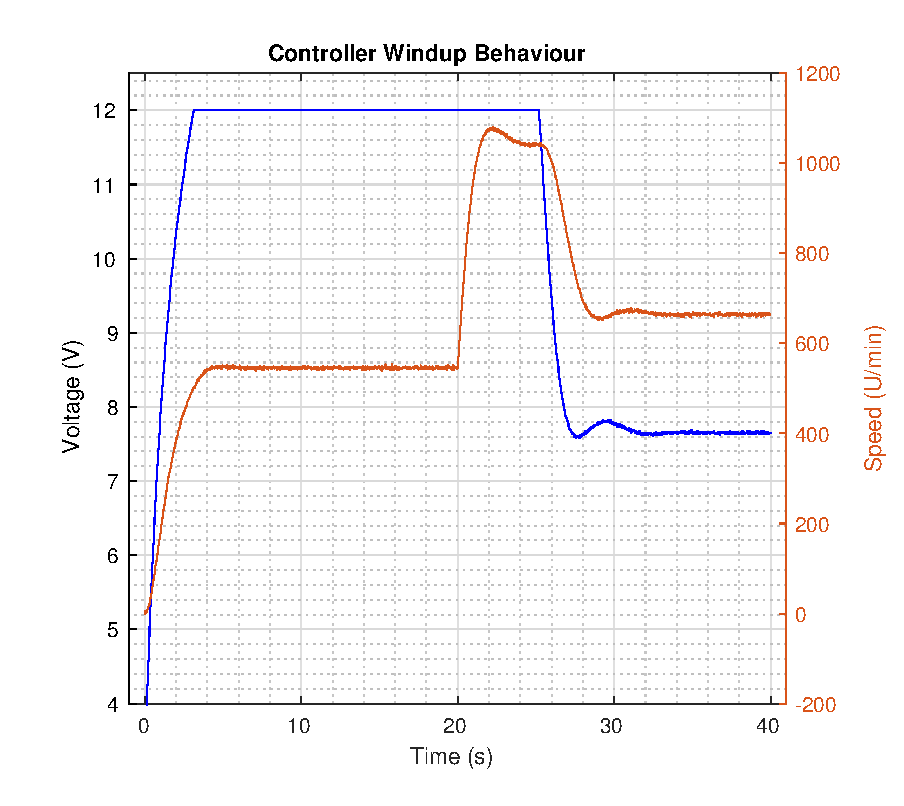
\includegraphics[width=\imagewidth]{images/windup}
    \caption{``\textit{Windup}''-Verhalten des Reglers. Bei $t=\SI{20}{\second}$ wird die Last entfernt, aber die Spannung bleibt eine Zeit lang bei \SI{12}{\volt} h\"angen.}
    \label{fig:windup}
\end{figure}

Eine L\"osung dazu ist den Integralteil zu limitieren. Die  gleiche Simulation
wird    durchgef\"uhrt,    aber   diesmal    ist    der    Integralteil    auf
\SI{0}{\volt}-\SI{12}{\volt} limitiert.

Wir    sehen    ein    viel    besseres    Verhalten    in    der    Abbildung
\ref{fig:windup_clamping}. Der Regler reagiert sofort  auf  die Last\"anderung
und bleibt nicht mehr eine weile lang stecken.

\begin{figure}[H]
    \centering
    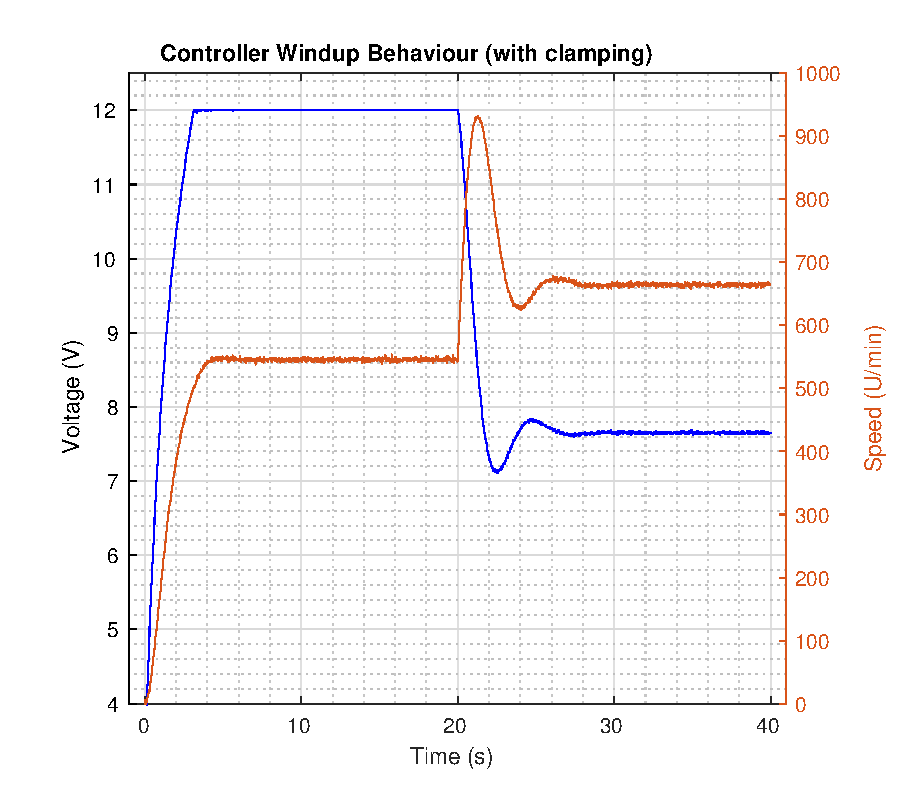
\includegraphics[width=\imagewidth]{images/windup_clamping}
    \caption{``\textit{Windup}''-Verhalten des Reglers. Bei $t=\SI{20}{\second}$ wird die Last entfernt und der Regler reagiert sofort.}
    \label{fig:windup_clamping}
\end{figure}


\subsection{Lastabh\"angigkeit}

Die  Abbildung  \ref{fig:target_500_load_0-10}  zeigt die  Schrittantwort  des
Systems mit einer Soll-Drehzahl von 500  U/min  bei  verschiedener  Last.  Die
L\"aste    sind    von    \SI{0}{\newton\meter\per(\radian\per\second)}    bis
\SI{0.01}{\newton\meter\per(\radian\per\second)} verteilt.

\begin{figure}[H]
    \centering
    \includegraphics[width=\imagewidth]{images/target_500_load_0-10}
    \caption{Verhalten bei einem Sollwert von 500 U/min und verschiedene L\"aste von 0 bis \SI{0.01}{\newton\meter\per(\radian\per\second)}. Der Sollwert wird erreicht, aber erst nach ca. \SI{10}{\second}!}
    \label{fig:target_500_load_0-10}
\end{figure}

Wie erwartet, muss der Regler eine h\"ohere Spannung erzeugen f\"ur zunehmende
Last.     Der     Schrittantwort     h\"ort     bei     einer     Last     von
$>\SI{0.003}{\newton\meter\per(\radian\per\second)}$  auf zu  \"uberschwingen.
Je h\"oher die Last, desto l\"anger hat das System, den Sollwert zu erreichen.


\subsection{Dynamisches Verhalten}

Die  Abbildung  \ref{fig:target_500_dynamic_load}  zeigt   das  Verhalten  des
Systems, wenn eine Last pl\"otzlich anf\"angt  zu  wirken, und nach einer Zeit
wieder aufh\"ohrt zu wirken.

\begin{figure}[H]
    \centering
    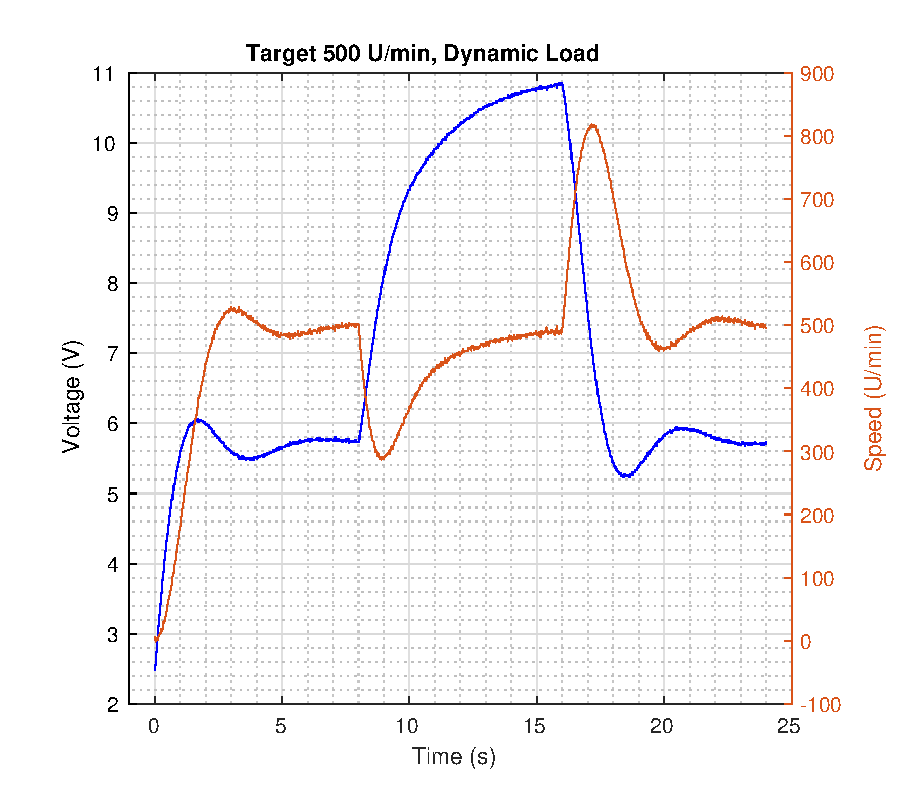
\includegraphics[width=\imagewidth]{images/target_500_dynamic_load}
    \caption{Verhalten bei einem Sollwert von 500 U/min und eine Last, die pl\"otzlich bei $t=\SI{8}{\second}$ wirkt und bei $t=\SI{16}{\second}$ wieder entfernt wird. Die Last entspricht \SI{0.01}{\newton\meter\per(\radian\per\second)}}
    \label{fig:target_500_dynamic_load}
\end{figure}

Die Last  betr\"agt dabei \SI{0.01}{\newton\meter\per(\radian\per\second)} und
f\"angt bei $t=\SI{8}{\second}$ an zu  wirken.  Bei  $t=\SI{16}{\second}$ wird
die Last wieder entfernt.

Wir sehen, dass der Motor  recht  stark  vom  Sollwert  schwankt  (etwa um 300
U/min).

